\documentclass{beamer}
\usetheme{Madrid}
\usepackage{amsmath}
\usepackage{siunitx}
\usepackage{tikz}
\usepackage{pgfplots}
\usepackage{apacite}
\pgfplotsset{compat=1.18}

\title{Comparison of Water Conservation in Dubai and in Singapore}
\subtitle{\small ESS SL Presentation}
\author{Eric}
%\institute{Ningbo Xiaoshi HS}
\date{\today}


\begin{document}

\begin{frame}
    \titlepage
\end{frame}

\begin{frame}{Table of Contents}
    \tableofcontents
\end{frame}

\section{Dubai Geographical Background}

\begin{frame}{Dubai Geographical Background-Location}

    \begin{figure}
        \centering
        \includegraphics[width = 0.5\textwidth]{imgs/climatemap.png}
        \caption{Location of Dubai, UAE}
        
        \small\cite{peel-2007}
    \end{figure}

\end{frame}

\begin{frame}{Dubai Geographical Background-Climate}

    \begin{figure}
        \centering
        \includegraphics[width = 0.5\textwidth]{imgs/climate-graph.png}
        \caption{Climate of Dubai, UAE}
        
        \small\cite{climategraph}
    \end{figure}
\end{frame}

\section{Singapore Geographical Background}

\begin{frame}{Singapore Geographical Background-Location}

    \begin{figure}
        \centering
        \includegraphics[width = 0.5\textwidth]{imgs/climatemap2.png}
        \caption{Location of Singapore}
        
        \small\cite{peel-2007}
    \end{figure}

\end{frame}

\begin{frame}{Singapore Geographical Background-Climate}

    \begin{figure}
        \centering
        \includegraphics[width = 0.5\textwidth]{imgs/climate-graph2.png}
        \caption{Climate of Singapore}
        
        \small\cite{climategraph}
    \end{figure}
\end{frame}

\section{Water resources}

\subsection{Scarcity}

\begin{frame}{Water resources - Comparison}
    \begin{itemize}
        \item Water is scarce in both place.
        \item But they are scarce and managed in different ways.
    \end{itemize}
\end{frame}

\subsection{Use of the renewable source}

\begin{frame}{Water resources - Use of the renewable source}
    \begin{columns}
    \begin{column}{0.48\textwidth}
    \begin{block}{Dubai}
        \begin{itemize}
            \item Authorities (e.g., DEWA) publish technical handbooks
            \item Implementing programmes
            \item National policies also call for rationalizing water consumption 
            \item Overall per-capita use remains high.
        \end{itemize}
        \cite{UAEhandbk}
    \end{block}
    \end{column}
    \begin{column}{0.48\textwidth}
    \begin{block}{Singapore}
        \begin{itemize}
            \item Strong regulatory and market tools
            \item Mandatory water-efficiency regulations
            \item Public education campaigns
            \item NEWater
            \item Low total cost per capita
        \end{itemize}
        \cite{SGwaterloop}
    \end{block}
    \end{column}
    \end{columns}
\end{frame}

\subsection{Reuse and recycling of waste}

\begin{frame}{Water resources - Reuse and recycling of waste water}
    \begin{columns}
    \begin{column}{0.48\textwidth}
    \begin{block}{Dubai}
        \begin{itemize}
            \item Desalination
            \item large multi-stage flash (MSF) and reverse osmosis (RO) desalination capacity
            \item Wastewater reuse / recycling targets 
            \item Reclaimed water (irrigation, industrial uses etc.)
        \end{itemize}
        \cite{SmartWater}
    \end{block}
    \end{column}
    \begin{column}{0.48\textwidth}
    \begin{block}{Singapore}
        \begin{itemize}
            \item NEWater (recycled high-grade reclaimed water)
            \item Used for industry and blended into reservoirs
            \item Desalination
            \item Import from other countries (e.g., Malaysia)
        \end{itemize}
        \cite{SGwaterloop}
    \end{block}
    \end{column}
    \end{columns}
\end{frame}

\section{City planning} %Shit there is too much I cant take it no more. 

\begin{frame}{City planning}
    
    \begin{figure}
        \centering
        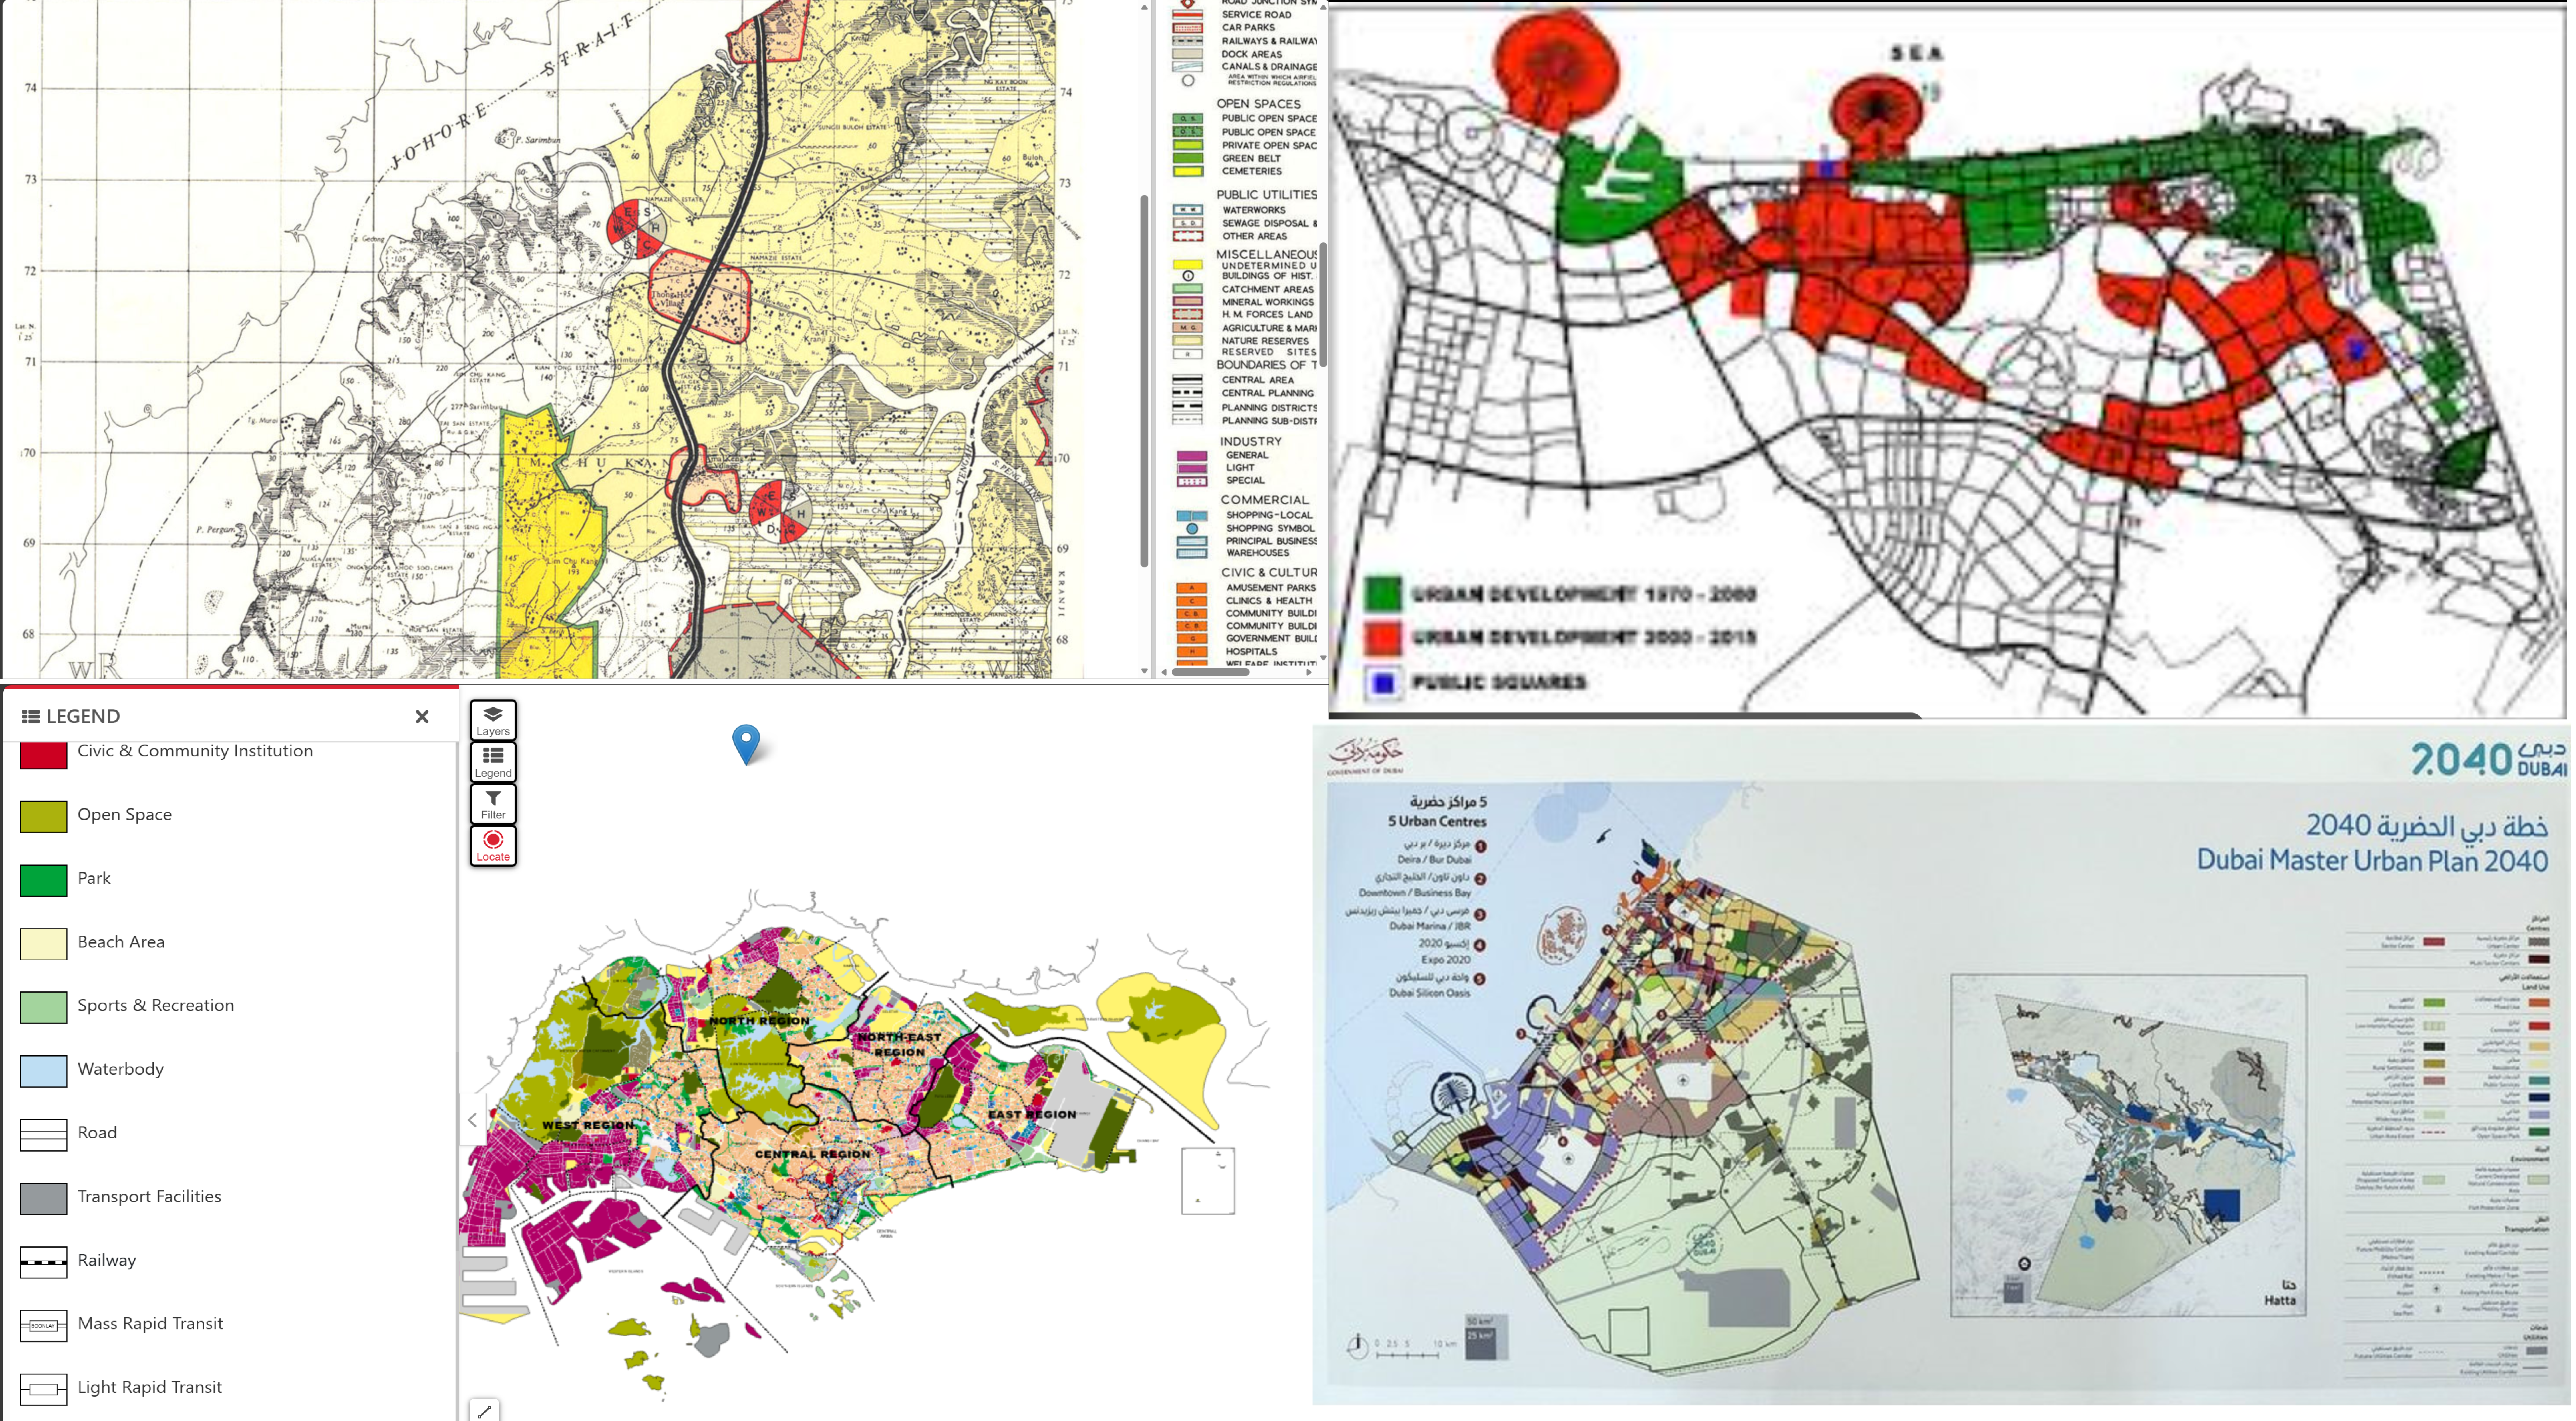
\includegraphics[width = 0.95\textwidth]{imgs/cp.png}
        \caption{City plannings}
        \small\cite{SG1958,SG2019, duabaiplan}
    \end{figure}
\end{frame}

\begin{frame}[allowframebreaks]{References}
    \bibliographystyle{apacite}
    \bibliography{cit.bib}
\end{frame}

\end{document}
